\documentclass{beamer}
\usetheme{Madrid}
\usepackage{tikz}
\usetikzlibrary{shapes}

\title{Analogical Reasoning}
\subtitle{How Humans Make Sense of the World}
\author{Brendan Shea, PhD}
\date{Introduction to Logic}

\begin{document}
	
	% Slide 1: Title Slide
	\frame{\titlepage}
	
	% Slide 2: Course Overview
	\begin{frame}{Lesson Overview: From Pattern Recognition to AI}
		\begin{itemize}
			\item This lesson explores how humans use \textbf{analogical reasoning} - the process of understanding new situations by comparing them to familiar ones.
			\item We will examine why the human mind naturally thinks in analogies and how this shapes our understanding across different domains.
			\item You will learn to evaluate what makes analogies effective or misleading in science, ethics, and law.
			\item We conclude by comparing human analogical thinking with AI pattern recognition systems.
		\end{itemize}
		
		\begin{alertblock}{Core Question}
			What makes some analogies powerful tools for understanding while others lead us astray?
		\end{alertblock}
	\end{frame}
	
	% Slide 3: The Cognitive Architecture of Analogy-Making
	\begin{frame}{The Cognitive Architecture of Analogy-Making}
		\begin{itemize}
			\item The human brain contains specialized regions that automatically search for \textbf{structural similarities} between different situations.
			\item \textbf{Working memory} allows us to hold multiple concepts simultaneously and map relationships between them.
			\item Our cognitive system prioritizes \textbf{relational matches} over surface features when making analogies.
			\item This architecture evolved because recognizing patterns across contexts provides survival advantages.
		\end{itemize}
		
		\begin{block}{Key Components}
			\begin{enumerate}
				\item Pattern detection systems
				\item Relational mapping processes
				\item Similarity evaluation mechanisms
			\end{enumerate}
		\end{block}
	\end{frame}
	
	% Slide 4: Why Our Brains Default to Analogical Thinking
	\begin{frame}{Why Our Brains Default to Analogical Thinking}
		\begin{itemize}
			\item Analogical thinking allows us to apply \textbf{previous knowledge} to novel situations without starting from scratch.
			\item It serves as a \textbf{cognitive shortcut} that saves mental energy and processing time.
			\item This default mode helps us navigate uncertainty by finding familiar patterns in unfamiliar contexts.
			\item \textbf{Evolutionary pressure} favored minds that could quickly recognize "this is like that" for rapid decision-making.
		\end{itemize}
		
		\begin{example}
			When early humans encountered a new predator, recognizing it as "like a lion" triggered appropriate defensive responses without direct experience.
		\end{example}
	\end{frame}
	
	% Slides 5-8 continue here...
	
	% Additional Slide: Everyday Examples of Analogical Reasoning
	\begin{frame}{Everyday Examples of Analogical Reasoning}
		\begin{itemize}
			\item \textbf{Learning}: "Multiplication is just repeated addition" helps students understand a new operation through a familiar one.
			\item \textbf{Communication}: "The internet is like a highway" explains data flow using traffic and routes.
			\item \textbf{Problem-solving}: "This math problem is like the one we did yesterday" recognizes similar structure despite different numbers.
			\item \textbf{Social understanding}: "She's going through what I went through last year" applies personal experience to understand others.
		\end{itemize}
		
		\begin{example}
			When teaching fractions, we say "cutting a pizza into slices" because:
			\begin{itemize}
				\item Source: Pizza (familiar, concrete)
				\item Target: Fractions (abstract, new)
				\item Mapping: Whole pizza = 1, slices = parts, sharing = division
			\end{itemize}
		\end{example}
	\end{frame}
	
	% Slide 5: Pattern Recognition and the Evolution of Reasoning
	\begin{frame}{Pattern Recognition and the Evolution of Reasoning}
		\begin{itemize}
			\item \textbf{Pattern recognition} emerged as a fundamental survival skill in early organisms detecting regularities in their environment.
			\item Human reasoning evolved from simple stimulus-response patterns to complex \textbf{abstract pattern matching}.
			\item Our ancestors who could recognize that "dark clouds mean rain" gained advantages in planning and resource management.
			\item This capacity expanded from physical patterns to social, causal, and conceptual patterns over evolutionary time.
		\end{itemize}
		
		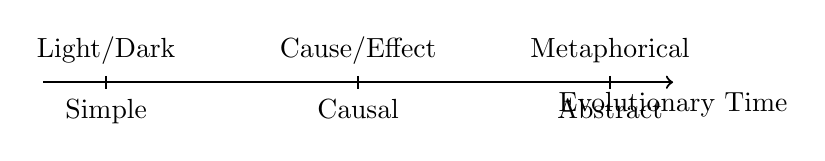
\begin{tikzpicture}[scale=0.8]
			\draw[thick,->] (0,0) -- (10,0) node[anchor=north] {Evolutionary Time};
			\draw[thick] (1,0.1) -- (1,-0.1) node[anchor=north] {Simple};
			\draw[thick] (5,0.1) -- (5,-0.1) node[anchor=north] {Causal};
			\draw[thick] (9,0.1) -- (9,-0.1) node[anchor=north] {Abstract};
			\node at (1,0.5) {Light/Dark};
			\node at (5,0.5) {Cause/Effect};
			\node at (9,0.5) {Metaphorical};
		\end{tikzpicture}
	\end{frame}
	
	% Slide 6: From Metaphor to Model: The Spectrum of Analogical Thought
	\begin{frame}{From Metaphor to Model: The Spectrum of Analogical Thought}
		\begin{itemize}
			\item Analogical thinking exists on a spectrum from loose \textbf{metaphors} to precise \textbf{scientific models}.
			\item \textbf{Metaphors} highlight selected similarities while ignoring differences (e.g., "time is money").
			\item \textbf{Analogies} make explicit comparisons between domains to explain or argue (e.g., "the heart is like a pump").
			\item \textbf{Models} systematically map multiple relationships from one domain to another (e.g., the planetary model of the atom).
		\end{itemize}
		
		\begin{block}{Increasing Precision}
			\begin{tabular}{l|l|l}
				\textbf{Type} & \textbf{Purpose} & \textbf{Rigor} \\
				\hline
				Metaphor & Illuminate & Low \\
				Analogy & Explain/Argue & Medium \\
				Model & Predict/Test & High
			\end{tabular}
		\end{block}
	\end{frame}
	
	% Slide 7: Anatomy of an Analogy: Source, Target, and Mapping
	\begin{frame}{Anatomy of an Analogy: Source, Target, and Mapping}
		\begin{itemize}
			\item Every analogy contains a \textbf{source domain} (the familiar concept) and a \textbf{target domain} (the unfamiliar concept being explained).
			\item The \textbf{mapping} identifies which elements in the source correspond to elements in the target.
			\item Strong analogies preserve \textbf{structural relationships} between elements, not just surface features.
			\item The process involves selecting relevant features while ignoring irrelevant differences between domains.
		\end{itemize}
		
		\begin{example}
			\textbf{Analogy}: "The atom is like a solar system"
			\begin{itemize}
				\item Source: Solar system (familiar)
				\item Target: Atom (unfamiliar)
				\item Mapping: Sun → nucleus, planets → electrons, orbits → electron paths
			\end{itemize}
		\end{example}
	\end{frame}
	
	% Slide 8: Structural Alignment: When Relationships Matter More Than Objects
	\begin{frame}{Structural Alignment: When Relationships Matter More Than Objects}
		\begin{itemize}
			\item \textbf{Structural alignment} means matching the relationships between elements rather than the elements themselves.
			\item Good analogies preserve \textbf{higher-order relations} - relationships between relationships.
			\item Surface similarities (color, size, shape) are less important than \textbf{relational structure} (causation, proportion, function).
			\item This principle explains why "the mind is a computer" works better than "the mind is a filing cabinet."
		\end{itemize}
		
		\begin{alertblock}{Key Insight}
			The power of an analogy lies not in how similar things look, but in how similarly they behave or relate to other elements in their respective systems.
		\end{alertblock}
	\end{frame}
	
	% Slides 9-12 continue here...
	
	% Slide 9: Surface vs. Deep Features in Analogical Reasoning
	\begin{frame}{Surface vs. Deep Features in Analogical Reasoning}
		\begin{itemize}
			\item \textbf{Surface features} are immediately observable characteristics like appearance, color, or size.
			\item \textbf{Deep features} involve underlying relationships, functions, or causal structures.
			\item Novices tend to focus on surface similarities, while experts recognize deep structural patterns.
			\item Effective analogical reasoning requires looking past superficial resemblance to find meaningful connections.
		\end{itemize}
		
		\begin{alertblock}{Common Mistake}
			Students often group physics problems by surface features (inclined planes, pulleys) rather than deep principles (conservation of energy, Newton's laws).
		\end{alertblock}
	\end{frame}
	
	% Slide 10: The Role of Context in Analogical Transfer
	\begin{frame}{The Role of Context in Analogical Transfer}
		\begin{itemize}
			\item \textbf{Context} determines which features of an analogy are relevant and which should be ignored.
			\item The same source can map to different targets depending on the \textbf{purpose} of the comparison.
			\item \textbf{Pragmatic constraints} shape how we interpret and apply analogies in real situations.
			\item Cultural background influences which analogies feel natural or forced to different audiences.
		\end{itemize}
		
		\begin{example}
			"Life is a journey" emphasizes different aspects in different contexts:
			\begin{itemize}
				\item Career counseling: progression, milestones, destinations
				\item Grief counseling: rough roads, companions, continuing forward
				\item Education: exploration, discovery, growth
			\end{itemize}
		\end{example}
	\end{frame}
	
	% Slide 11: Criteria for Evaluating Analogical Arguments
	\begin{frame}{Criteria for Evaluating Analogical Arguments}
		\begin{itemize}
			\item \textbf{Relevance}: The shared properties must be relevant to the conclusion being drawn.
			\item \textbf{Quantity}: More similarities generally strengthen an analogy, but quality matters more than quantity.
			\item \textbf{Diversity}: Similarities across different types of features provide stronger support.
			\item \textbf{Disanalogy}: Important differences between source and target can weaken or defeat the argument.
		\end{itemize}
		
		\begin{block}{Evaluation Checklist}
			\begin{enumerate}
				\item Are the similarities relevant to the conclusion?
				\item Do the differences matter for this purpose?
				\item Is the source well-understood?
				\item Are there alternative analogies to consider?
			\end{enumerate}
		\end{block}
	\end{frame}
	
	% Slide 12: Relevant Similarities and the Problem of Selection
	\begin{frame}{Relevant Similarities and the Problem of Selection}
		\begin{itemize}
			\item Any two things share infinite similarities and differences, creating a \textbf{selection problem}.
			\item \textbf{Relevance} depends on the specific claim or conclusion the analogy supports.
			\item We must identify which shared features actually matter for the \textbf{inferential goal}.
			\item Background knowledge and theory guide us in selecting appropriate features to compare.
		\end{itemize}
		
		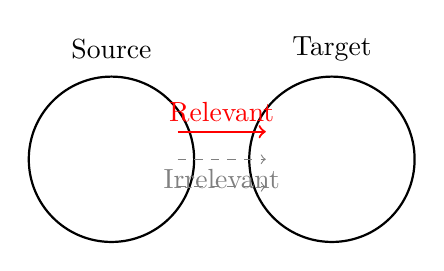
\begin{tikzpicture}[scale=0.7]
			% Draw two circles
			\draw[thick] (2,0) circle (1.5cm);
			\node at (2,2) {Source};
			\draw[thick] (6,0) circle (1.5cm);
			\node at (6,2) {Target};
			
			% Draw arrows between them
			\draw[->, thick, red] (3.2,0.5) -- (4.8,0.5) node[midway, above] {Relevant};
			\draw[->, dashed, gray] (3.2,0) -- (4.8,0) node[midway, below] {Irrelevant};
			\draw[->, dashed, gray] (3.2,-0.5) -- (4.8,-0.5);
		\end{tikzpicture}
	\end{frame}
	
	% Slides 13-16 continue here...
	
	% Slide 13: When Dissimilarities Matter: Negative Analogy
	\begin{frame}{When Dissimilarities Matter: Negative Analogy}
		\begin{itemize}
			\item \textbf{Negative analogy} refers to the ways in which the source and target differ.
			\item Some differences are harmless to the analogy, while others are \textbf{defeaters} that undermine the comparison.
			\item A difference becomes critical when it affects the specific relationship or property being transferred.
			\item Recognizing relevant dissimilarities helps us avoid overextending analogies beyond their useful scope.
		\end{itemize}
		
		\begin{alertblock}{Critical Question}
			Does this difference break the relationship I'm trying to map from source to target?
		\end{alertblock}
	\end{frame}
	
	% Slide 14: The Danger of Superficial Resemblance
	\begin{frame}{The Danger of Superficial Resemblance}
		\begin{itemize}
			\item \textbf{Superficial resemblance} occurs when things look similar but lack deep structural correspondence.
			\item This mistake often leads to false predictions and poor decision-making.
			\item Marketing and propaganda frequently exploit surface similarities to create misleading associations.
			\item Training in analogical reasoning helps us resist being fooled by mere appearance.
		\end{itemize}
		
		\begin{example}
			\textbf{Misleading Analogy}: "This alternative medicine works like traditional medicine"
			\begin{itemize}
				\item Surface similarity: Both come in pill form
				\item Missing deep structure: No tested biological mechanism
				\item Result: False confidence in effectiveness
			\end{itemize}
		\end{example}
	\end{frame}
	
	% Slide 15: Historical Examples: From Plato's Cave to Darwin's Tree
	\begin{frame}{Historical Examples: From Plato's Cave to Darwin's Tree}
		\begin{itemize}
			\item \textbf{Plato's Cave}: Reality is to shadows as true knowledge is to sensory experience.
			\item \textbf{Newton's Clockwork Universe}: The cosmos operates like a precise mechanical clock.
			\item \textbf{Darwin's Tree of Life}: Species relationships branch like a growing tree.
			\item \textbf{Freud's Iceberg}: Conscious thought is the tip; the unconscious lies beneath.
		\end{itemize}
		
		\begin{block}{Why These Analogies Endured}
			These analogies succeeded because they:
			\begin{itemize}
				\item Mapped complex abstract ideas to concrete images
				\item Preserved crucial relationships
				\item Generated testable predictions
			\end{itemize}
		\end{block}
	\end{frame}
	
	% Slide 16: Everyday Analogies We Live By
	\begin{frame}{Everyday Analogies We Live By}
		\begin{itemize}
			\item \textbf{Time is money}: We "spend," "save," "waste," and "invest" time.
			\item \textbf{Arguments are war}: We "defend" positions, "attack" weak points, and "win" debates.
			\item \textbf{Ideas are food}: We "digest" information, "chew on" problems, and find some ideas "hard to swallow."
			\item \textbf{Organizations are organisms}: Companies "grow," have "healthy" cultures, and can "die."
		\end{itemize}
		
		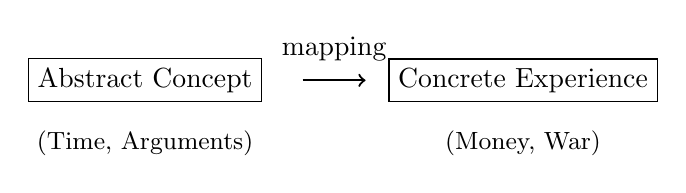
\begin{tikzpicture}[scale=0.8]
			\node[draw, rectangle] at (0,0) {Abstract Concept};
			\node[draw, rectangle] at (6,0) {Concrete Experience};
			\draw[->, thick] (2.5,0) -- (3.5,0);
			\node at (3,0.5) {mapping};
			\node at (0,-1) {\small (Time, Arguments)};
			\node at (6,-1) {\small (Money, War)};
		\end{tikzpicture}
	\end{frame}
	
	% Slides 17-20 continue here...
	
	% Slide 17: Models as Extended Analogies in Scientific Discovery
	\begin{frame}{Models as Extended Analogies in Scientific Discovery}
		\begin{itemize}
			\item Scientific \textbf{models} are systematic analogies that map multiple relationships from familiar to unfamiliar domains.
			\item Unlike simple analogies, models generate \textbf{quantitative predictions} that can be tested experimentally.
			\item Scientists use models as \textbf{thinking tools} to explore implications and design new experiments.
			\item The best models reveal unexpected connections and suggest new research directions.
		\end{itemize}
		
		\begin{block}{From Analogy to Model}
			\begin{tabular}{l|l}
				\textbf{Simple Analogy} & \textbf{Scientific Model} \\
				\hline
				"Heart is like a pump" & Cardiac pressure equations \\
				"Brain is like a computer" & Neural network algorithms \\
				"DNA is like a code" & Base-pair transcription rules
			\end{tabular}
		\end{block}
	\end{frame}
	
	% Slide 18: Case Study: The Wave-Particle Duality of Light
	\begin{frame}{Case Study: The Wave-Particle Duality of Light}
		\begin{itemize}
			\item Scientists initially debated whether light was analogous to \textbf{water waves} or \textbf{flying particles}.
			\item Wave analogy explained: interference patterns, diffraction, and refraction phenomena.
			\item Particle analogy explained: photoelectric effect and discrete energy packets.
			\item The resolution required accepting that light doesn't perfectly match either familiar analogy.
		\end{itemize}
		
		\begin{example}
			The double-slit experiment revealed the limitation of classical analogies:
			\begin{itemize}
				\item Individual photons (particle-like) create interference patterns (wave-like)
				\item Neither waves nor particles from everyday experience behave this way
				\item New quantum framework transcended both analogies
			\end{itemize}
		\end{example}
	\end{frame}
	
	% Slide 19: When Scientific Analogies Mislead: The Ether Hypothesis
	\begin{frame}{When Scientific Analogies Mislead: The Ether Hypothesis}
		\begin{itemize}
			\item 19th-century physicists assumed light waves needed a \textbf{medium} like sound waves need air.
			\item They invented "luminiferous ether" by analogy to other wave phenomena.
			\item This analogy led to decades of failed experiments searching for ether's properties.
			\item The Michelson-Morley experiment finally showed the analogy was fundamentally flawed.
		\end{itemize}
		
		\begin{alertblock}{Lesson Learned}
			Even productive analogies have limits - scientific progress often requires abandoning familiar comparisons for genuinely new concepts.
		\end{alertblock}
	\end{frame}
	
	% Slide 20: Thought Experiments as Analogical Tools
	\begin{frame}{Thought Experiments as Analogical Tools}
		\begin{itemize}
			\item \textbf{Thought experiments} use imaginative analogies to explore logical consequences of theories.
			\item They allow scientists to test ideas when real experiments are impossible or impractical.
			\item Famous examples include Einstein's elevator, Schrödinger's cat, and Maxwell's demon.
			\item These analogical scenarios reveal hidden assumptions and paradoxes in our theories.
		\end{itemize}
		
		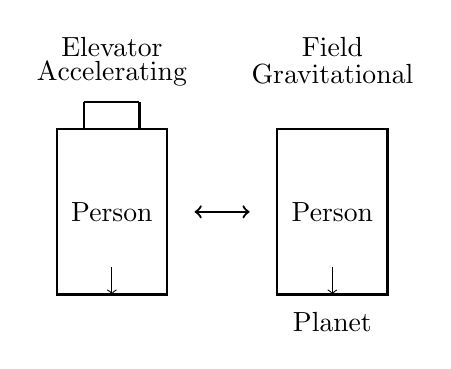
\begin{tikzpicture}[scale=0.7]
			% Draw a simple elevator diagram
			\draw[thick] (0,0) rectangle (2,3);
			\draw[thick] (0.5,3) -- (0.5,3.5);
			\draw[thick] (1.5,3) -- (1.5,3.5);
			\draw[thick] (0.5,3.5) -- (1.5,3.5);
			\node at (1,1.5) {Person};
			\draw[->] (1,0.5) -- (1,0);
			
			\draw[thick] (4,0) rectangle (6,3);
			\node at (5,1.5) {Person};
			\draw[->] (5,0.5) -- (5,0);
			\node at (5,-0.5) {Planet};
			
			\node at (1,4) {Accelerating};
			\node at (1,4.5) {Elevator};
			\node at (5,4) {Gravitational};
			\node at (5,4.5) {Field};
			
			\draw[<->, thick] (2.5,1.5) -- (3.5,1.5);
		\end{tikzpicture}
	\end{frame}
	
	% Slides 21-24 continue here...
	
	% Slide 21: The Computer Model of Mind: Strengths and Limitations
	\begin{frame}{The Computer Model of Mind: Strengths and Limitations}
		\begin{itemize}
			\item The \textbf{computational theory of mind} treats mental processes as information processing operations.
			\item Strengths: Explains memory storage, logical reasoning, and step-by-step problem solving.
			\item Limitations: Struggles with consciousness, emotions, and contextual understanding.
			\item This analogy revolutionized cognitive science but may constrain how we think about minds.
		\end{itemize}
		
		\begin{block}{Mapping the Analogy}
			\begin{itemize}
				\item Hardware → Brain structure
				\item Software → Mental processes
				\item Input/Output → Perception/Action
				\item Bugs → Mental disorders (problematic?)
			\end{itemize}
		\end{block}
	\end{frame}
	
	% Slide 22: DNA as Code: A Productive Metaphor
	\begin{frame}{DNA as Code: A Productive Metaphor}
		\begin{itemize}
			\item The \textbf{genetic code} analogy helped scientists understand how DNA stores and transmits information.
			\item \textit{DNA is like an instruction book (or computer program) for building proteins. Genes are like chapters.}
			\item This framing led to breakthroughs in sequencing, gene editing, and synthetic biology.
			\item The analogy suggests we can "debug" genetic diseases and "reprogram" organisms.
			\item However, biological systems are messier than computer code, with complex feedback loops.
		\end{itemize}
		
		\begin{example}
			\scriptsize
			Successful predictions from the code analogy:
			\begin{itemize}
				\item Four-letter alphabet (A, T, G, C) → words (codons) → sentences (genes)
				\item Copy errors → mutations
				\item Reading frames → translation mechanisms
			\end{itemize}
		\end{example}
	\end{frame}
	
	% Slide 23: Moral Reasoning Through Analogical Cases
	\begin{frame}{Moral Reasoning Through Analogical Cases}
		\begin{itemize}
			\item Ethical reasoning often proceeds by finding \textbf{analogous cases} where our intuitions are clearer.
			\item We test moral principles by applying them to similar situations and checking for consistency.
			\item \textbf{Case-based reasoning} helps us navigate novel ethical dilemmas using established precedents.
			\item The challenge lies in determining which features are morally relevant for comparison.
		\end{itemize}
		
		\begin{alertblock}{Key Ethical Question}
			If we accept X in situation A, must we also accept Y in analogous situation B?
		\end{alertblock}
	\end{frame}
	
	% Slide 24: The Trolley Problem and Its Analogical Extensions
	\begin{frame}{The Trolley Problem and Its Analogical Extensions}
		\begin{itemize}
			\item The \textbf{trolley problem} uses a concrete scenario to explore abstract principles about harm and intention.
			\item \textit{Suppose a runaway trolley is headed toward five workers--it will kill them if not stopped. You are standing near a switch that will redirect this trolley so it kills one worker on a different track instead.}
			\item Variations test our intuitions: switching tracks vs. pushing someone, acting vs. allowing harm.
			\item These thought experiments reveal tensions between \textbf{utilitarian} and \textbf{deontological} ethics.
			\item Real-world applications include medical triage, autonomous vehicles, and military decisions.
		\end{itemize}
		
		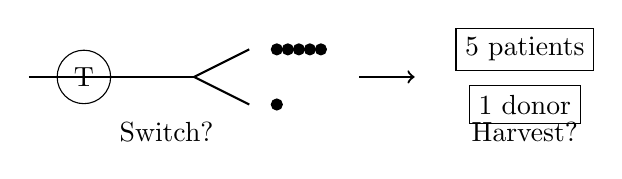
\begin{tikzpicture}[scale=0.7]
			% Original trolley problem
			\draw[thick] (0,1) -- (3,1);
			\draw[thick] (3,1) -- (4,1.5);
			\draw[thick] (3,1) -- (4,0.5);
			\node[draw, circle] at (1,1) {T};
			\draw[fill=black] (4.5,1.5) circle (0.1);
			\draw[fill=black] (4.7,1.5) circle (0.1);
			\draw[fill=black] (4.9,1.5) circle (0.1);
			\draw[fill=black] (5.1,1.5) circle (0.1);
			\draw[fill=black] (5.3,1.5) circle (0.1);
			\draw[fill=black] (4.5,0.5) circle (0.1);
			\node at (2.5,0) {Switch?};
			
			% Arrow to analogous case
			\draw[->, thick] (6,1) -- (7,1);
			
			% Analogous medical case
			\node[draw, rectangle] at (9,1.5) {5 patients};
			\node[draw, rectangle] at (9,0.5) {1 donor};
			\node at (9,0) {Harvest?};
		\end{tikzpicture}
	\end{frame}
	
	% Slides 25-28 continue here...
	
	% Slide 25: Using Analogies to Expand Our Moral Circle
	\begin{frame}{Using Analogies to Expand Our Moral Circle}
		\begin{itemize}
			\item \textbf{Moral progress} often occurs when we recognize analogies between accepted and contested cases.
			\item Historical example: Arguments against slavery drew analogies to accepted rights of free persons.
			\item Contemporary debates use analogical extension: animal rights, AI rights, environmental protection.
			\item The \textbf{expanding circle} of moral concern relies on seeing similarities across boundaries.
		\end{itemize}
		
		\begin{block}{Pattern of Moral Expansion}
			\begin{enumerate}
				\item Establish principle for core case (humans deserve respect)
				\item Identify relevant similarity (capacity to suffer)
				\item Extend principle to analogous beings (animals can suffer too)
				\item Overcome resistance from surface differences
			\end{enumerate}
		\end{block}
	\end{frame}
	
	% Slide 26: When Ethical Analogies Break Down
	\begin{frame}{When Ethical Analogies Break Down}
		\begin{itemize}
			\item Ethical analogies fail when \textbf{morally relevant differences} are overlooked or minimized.
			\item False analogies can justify harmful actions by focusing on superficial similarities.
			\item Context and relationships matter: what works in one domain may not transfer to another.
			\item We must carefully examine whether the features that ground moral status are truly shared.
		\end{itemize}
		
		\begin{alertblock}{Warning Signs}
			An ethical analogy may be flawed when:
			\begin{itemize}
				\item It ignores power differentials
				\item It strips away important context
				\item It assumes universal values across cultures
				\item It oversimplifies complex relationships
			\end{itemize}
		\end{alertblock}
	\end{frame}
	
	% Slide 27: Animal Rights Arguments: From Human to Non-Human
	\begin{frame}{Animal Rights Arguments: From Human to Non-Human}
		\begin{itemize}
			\item Peter Singer's argument uses \textbf{analogical reasoning} to extend rights from humans to animals.
			\item Core analogy: If suffering matters morally for humans, it should matter for all sentient beings.
			\item The argument maps our obligations to vulnerable humans onto our treatment of animals.
			\item Critics challenge the analogy by pointing to cognitive differences and special human relationships.
		\end{itemize}
		
		\begin{example}
			Argument by analogy:
			\begin{itemize}
				\item We don't harm human infants (who lack full rationality)
				\item Adult pigs are more cognitively capable than human infants
				\item Therefore, the capacity difference doesn't justify harming pigs
				\item Conclusion: Species membership alone is arbitrary (speciesism)
			\end{itemize}
		\end{example}
	\end{frame}
	
	% Slide 28: The Violinist Argument in Bioethics
	\begin{frame}{The Violinist Argument in Bioethics}
		\begin{itemize}
			\item Judith Thomson's famous thought experiment uses \textbf{analogical reasoning} to examine abortion ethics.
			\item Scenario: You have been kidnapped by the Society of Music Lovers, and wake up connected to a famous unconscious (innocent) violinist who needs your kidneys for nine months.
			\item The analogy maps bodily autonomy rights from this case to specific pregnancy situations. perspective.
		\end{itemize}
		
		\begin{block}{Structure of the Argument}
			\begin{tabular}{l|l}
				\textbf{Violinist Case} & \textbf{Target Case} \\
				\hline
				Kidnapped person & Pregnant woman \\
				Unconscious violinist & Fetus \\
				Life support connection & Pregnancy \\
				Right to disconnect? & Right to terminate?
			\end{tabular}
		\end{block}
	\end{frame}
	
	% Slides 29-32 continue here...
	
	% Slide 29: Legal Precedent as Institutionalized Analogy
	\begin{frame}{Legal Precedent as Institutionalized Analogy}
		\begin{itemize}
			\item The \textbf{common law system} operates through analogical reasoning from case to case.
			\item \textbf{Stare decisis} ("let the decision stand") requires treating like cases alike.
			\item Lawyers argue by showing similarities to favorable precedents and differences from unfavorable ones.
			\item This system embeds analogical reasoning into the fundamental structure of legal decision-making.
		\end{itemize}
		
		\begin{block}{Legal Reasoning Process}
			\begin{enumerate}
				\item Identify relevant precedent cases
				\item Extract the legal principle (ratio decidendi)
				\item Map facts from precedent to current case
				\item Apply the principle if facts are sufficiently similar
			\end{enumerate}
		\end{block}
	\end{frame}
	
	% Slide 30: The Art of Distinguishing Cases
	\begin{frame}{The Art of Distinguishing Cases}
		\begin{itemize}
			\item \textbf{Distinguishing} means showing why a precedent doesn't apply to the current case.
			\item Lawyers must identify legally relevant differences between cases.
			\item The skill lies in determining which factual differences actually matter for the legal principle.
			\item Judges must balance consistency with precedent against adapting to new circumstances.
		\end{itemize}
		
		\begin{example}
			A lawyer might distinguish cases by arguing:
			\begin{itemize}
				\item "In \textit{Smith v. Jones}, the contract was verbal, but here it's written"
				\item This difference matters if the legal principle involves proof standards
				\item But wouldn't matter if the principle is about consideration
			\end{itemize}
		\end{example}
	\end{frame}
	
	% Slide 31: Ratio Decidendi: Finding the Relevant Similarities
	\begin{frame}{Ratio Decidendi: Finding the Relevant Similarities}
		\begin{itemize}
			\item \textbf{Ratio decidendi} is the legal principle that emerges from the essential facts of a case.
			\item Courts must determine which facts were crucial to the decision and which were incidental.
			\item Future cases are bound by the ratio, not by irrelevant details (\textbf{obiter dicta}).
			\item Different interpretations of the ratio lead to narrower or broader applications of precedent.
		\end{itemize}
		
		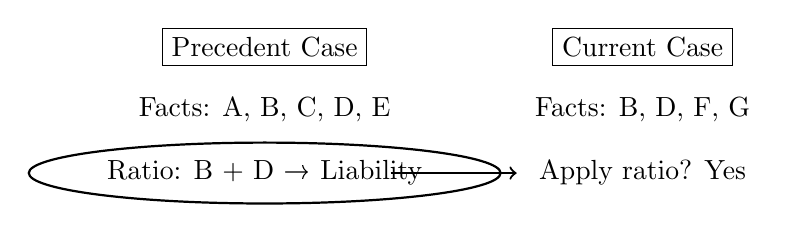
\begin{tikzpicture}[scale=0.8]
			% Draw a case with multiple facts
			\node[draw, rectangle] at (0,2) {Precedent Case};
			\node at (0,1) {Facts: A, B, C, D, E};
			\node[draw, ellipse, thick] at (0,0) {Ratio: B + D → Liability};
			
			% Arrow to new case
			\draw[->, thick] (2,0) -- (4,0);
			
			% New case
			\node[draw, rectangle] at (6,2) {Current Case};
			\node at (6,1) {Facts: B, D, F, G};
			\node at (6,0) {Apply ratio? Yes};
		\end{tikzpicture}
	\end{frame}
	
	% Slide 32: Landmark Cases and Their Analogical Legacy
	\begin{frame}{Landmark Cases and Their Analogical Legacy}
		\begin{itemize}
			\item \textbf{Landmark cases} establish principles that shape legal reasoning for generations.
			\item \textit{Brown v. Board}: "Separate but equal" fails because segregation inherently implies inequality.
			\item \textit{Miranda v. Arizona}: Custodial interrogation is inherently coercive without warnings.
			\item These cases become \textbf{source domains} for countless analogical arguments in new contexts.
		\end{itemize}
		
		\begin{alertblock}{Extending Landmark Principles}
			\textit{Brown's} equality principle has been analogically extended to:
			\begin{itemize}
				\item Gender discrimination in education
				\item Disability accommodations
				\item LGBTQ+ rights
				\item Each extension required arguing the analogy held
			\end{itemize}
		\end{alertblock}
	\end{frame}
	
	% Slides 33-36 continue here...
	
	% Slide 33: When New Technology Challenges Old Analogies
	\begin{frame}{When New Technology Challenges Old Analogies}
		\begin{itemize}
			\item Legal systems struggle when \textbf{new technologies} don't fit existing analogical frameworks.
			\item Courts must decide: Is the internet like a newspaper, a broadcast, or something entirely new?
			\item Cryptocurrency challenges analogies: Is it property, currency, a security, or a new category?
			\item Poor analogical choices can lead to decades of problematic legal precedents.
		\end{itemize}
		
		\begin{example}
			Email privacy case:
			\begin{itemize}
				\item Is email like a sealed letter (strong protection)?
				\item Or like a postcard (limited protection)?
				\item Or like a phone call (context-dependent)?
				\item The chosen analogy shapes privacy rights
			\end{itemize}
		\end{example}
	\end{frame}
	
	% Slide 34: How AI Systems Approach Pattern Matching
	\begin{frame}{How AI Systems Approach Pattern Matching}
		\begin{itemize}
			\item AI systems find patterns through \textbf{statistical correlation} rather than causal understanding.
			\item Machine learning identifies similarities in high-dimensional feature spaces.
			\item Unlike humans, AI doesn't rely on \textbf{structural mapping} or understanding relationships.
			\item AI can detect patterns humans miss but also make errors humans would never make.
		\end{itemize}
		
		\begin{block}{AI vs Human Pattern Recognition}
			\begin{tabular}{l|l}
				\textbf{Human Analogies} & \textbf{AI Pattern Matching} \\
				\hline
				Causal understanding & Statistical correlation \\
				Structural alignment & Feature similarity \\
				Context-sensitive & Context-agnostic \\
				Few examples needed & Many examples needed
			\end{tabular}
		\end{block}
	\end{frame}
	
	% Slide 35: Key Differences: Statistical Correlation vs. Causal Understanding
	\begin{frame}{Key Differences: Statistical Correlation vs. Causal Understanding}
		\begin{itemize}
			\item Humans use analogies to infer \textbf{causal mechanisms} from one domain to another.
			\item AI systems find \textbf{correlational patterns} without understanding why they exist.
			\item This difference explains why AI can be fooled by adversarial examples that wouldn't confuse humans.
			\item Understanding this distinction helps us use AI appropriately and recognize its limitations.
		\end{itemize}
		
		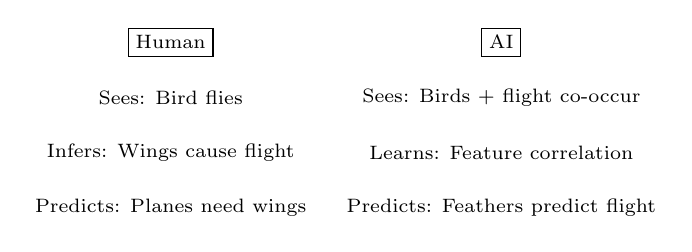
\begin{tikzpicture}[scale=0.7]
			\scriptsize
			% Human reasoning
			\node[draw] at (0,3) {Human};
			\node at (0,2) {Sees: Bird flies};
			\node at (0,1) {Infers: Wings cause flight};
			\node at (0,0) {Predicts: Planes need wings};
			
			% AI reasoning
			\node[draw] at (6,3) {AI};
			\node at (6,2) {Sees: Birds + flight co-occur};
			\node at (6,1) {Learns: Feature correlation};
			\node at (6,0) {Predicts: Feathers predict flight};
		\end{tikzpicture}
	\end{frame}
	
	% Slide 36: The Power and Peril of Thinking in Analogies
	\begin{frame}{The Power and Peril of Thinking in Analogies}
		\begin{itemize}
			\item Analogical reasoning is \textbf{fundamental} to human cognition and cultural progress.
			\item It enables us to leverage past experience, communicate abstract ideas, and make creative leaps.
			\item However, analogies can also constrain thinking, perpetuate biases, and mislead us.
			\item The key is developing \textbf{metacognitive awareness} about when and how we use analogies.
		\end{itemize}
		
		\begin{alertblock}{Final Takeaways}
			\begin{itemize}
				\item Recognize when you're reasoning by analogy
				\item Evaluate the structural mapping, not surface features
				\item Consider multiple analogies before committing
				\item Know when to abandon an analogy that no longer serves
			\end{itemize}
		\end{alertblock}
	\end{frame}
\end{document}